

\chapter{Introduction}\label{ch:intro}
\bigskip



\section{Purpose of the Project}

The \emph{OS Imaging System with Centralised Archiving and Distribution}
is an open source project based on open source tools made for the purpose
of optimising the imaging operations in environments such as school or
university laboratory with a network of workstations. It is built around
frameworks such as UDP Cast, an open source tool for system imaging and
Python, a popular programming language with many libraries  available.

The project plans to introduce features to the normal idea of an imaging
system, such as the possibility to archive and backup Operating System
Images and, most important, provide an always-available server with a
database of images.

The network infrastructure is built upon the Multicast protocol in IP.
This is used to optimise the traffic in the network by reducing the number
of unicast streams in the client-server model to a single multicast stream.

\section{The need for imaging systems}


Setting up a computer means two things: getting the hardware (a normal
PC) and installing a modern Operating System on it to control that
hardware. This is a job that would take a normal person, with basic
computer operating skills, about one hour on average. However, the
normal approach does not scale to installing on 3 or more hosts that
need the exact same setup.


In office environments, Internet/Game Cafes and, most important, in
school laboratories where 15 to 20 computers with identical
configuration need to be set up, an imaging solution is needed.  This
means that the setup will be done on a single computer and then, the
entire disk on which the new operating system resides is copied
throughout the network onto the disks of the other uninstalled hosts.
This can save, for a number of 20 hosts, from 20 hours of work to only
two hours (about one hour for installing one system and another hour
for the copy of the disk(s) over the network).


To get a perfect mirroring, it is recommended that the hosts be
identical (same CPU, same Main board, same \ac{HDD}s, same network card).
If the systems differ in a slight way, it is up to the operating
system to try and adapt to new hardware and install the appropriate
drivers.  From the operating system’s point of view, it is like the
HDD was taken out of one computer and installed in another one.

\begin{figure}[h]
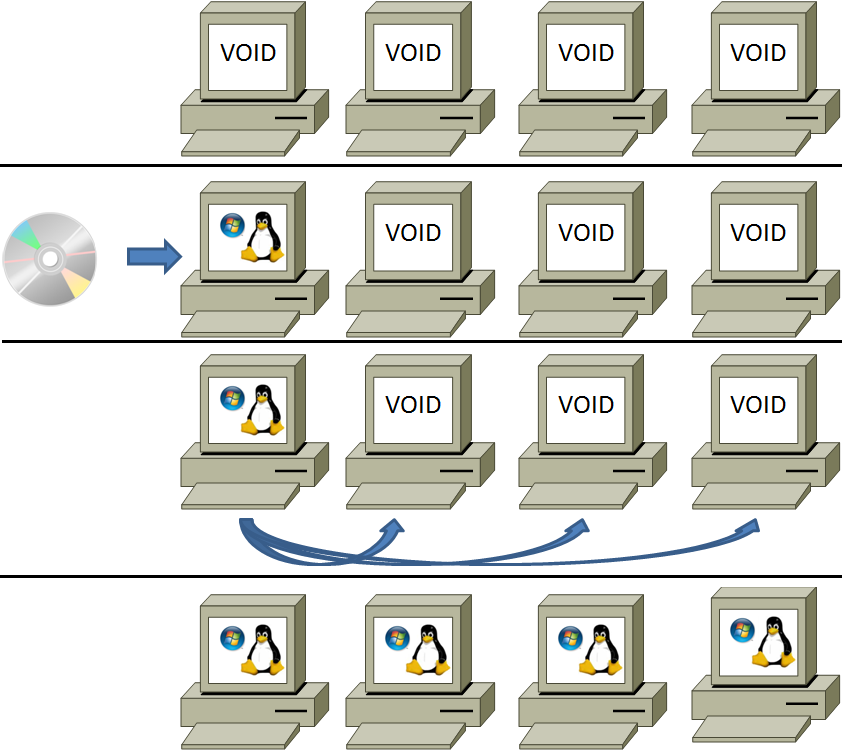
\includegraphics[width=10cm]{img/4comp}
\caption{Simple imaging operations}
\label{fig:4comp}
\end{figure}


To image a network of stations, there are some basic steps you need to take

\begin{enumerate}
\setcounter{enumi}{0}
\item Prepare all the hosts so they can power on. They can have empty
hard disks or hard disks with data that can be deleted.


\item Install one or more operating systems on one host.  This host will
be the seed host.  The operating system(s) can be personalized with
user accounts, installed programs, configured environments. Along with
the operating system(s), on the hard disk there will be the stage 1
boot loader in the \ac{MBR} and the upper stages of the boot loader on
other partitions. Separate partitions for personal data or backups can
be created


\item All the hosts must be able to boot in a pseudo-operating system
provided by the imaging software from a Live CD,  over the network via
PXE or from a local special partition so the working operating is not
modified during the imaging operation.


\item The contents of the seed’s hard disk are copied over the network
(usually using UDP over Multicast IP).  After the transfer is
complete, all hosts boot up normally.
\end{enumerate}



When using imaging systems, software licensing must be taken under
consideration.  The software that has per host or per CPU license has
to have a separate license code for each host.
There are two widely used software suits that provide system imaging:
Symatec Norton Ghost and UDP Cast. The first one is a professional
closed source enterprise software while the second one is an open
source project developed by a community.  Because of the flexibility
of open source projects, UDP cast, has been used in the development of
this imaging system solution and will be described in more detail.


